\section{Implementation and evaluation}\label{sec:implementation}
% 
In the prototype, we use the architecture described in Figure \ref{fig:arch-ver2-tech} as the basis for our system design. To be able to implement such a prototype, we need to break our idea down to a list of desired functions or functional requirements. Furthermore, the idea of this product includes some overall themes that the solution should follow, such as security and decentralisation. These \textit{themes} can be broken down to Non-functional requirements \acrshort{nfr}, which describe properties of the system.

\subsection{Prototype requirements}

In this section, we will describe the desired behaviour of the prototype using functional and non-functional requirements. In the first part, functional requirements are used to describe the intended functionality of the system as a whole, as seen from user's perspective. In the second part, we will capture some important characteristics that the system should have, using non-functional requirements.

\subsubsection{Functional requirements}
Usually, functional requirements would come from the users of the system, product owner and other stakeholders. In this project, the authors took the role of the product owner and envisioned the first set of requirements. This first set made up the prototype requirements. In further releases, users and other stakeholders would likely need to be considered.

% we list the requirements for the prototype, so that the idea can be demonstrated clearly. Requirements necessary for demonstrating the idea were prioritised, the others were not worked upon. We ranked the requirements by their importance and then sorted them in a MoSCoW table. We used this table to prioritise the areas for implementation. In a market-ready product, many requirements would most likely be different.

The idea of the system is to allow users trade Ether for another cryptocurrency, which is Bitcoin in this case. Both the user that sells Ether and buys Bitcoin (in previous chapter also referred to as \textit{Alice}) and the user that buys Ether and sells Bitcoin (previously referred to as \textit{Bob}) interact with the same application. For clarity, for the rest of this chapter, we will refer to the Ether selling user as \textit{primary user} and their trading partner (Ether buying user) as \textit{secondary user}.

The requirements for the prototype were selected in such way, so that the overall idea of the system can be demonstrated. The selection is demonstrated in Table \ref{tab:pt-func-reqs}. 

\begin{table}[ht]
    \centering
    \begin{tabularx}{\textwidth}{|l|X|}
    \hline
    \textbf{Requirement ID}& \textbf{Requirement text}\\
    \hline
    PT-FR-1 & The primary user and the secondary user should be able to agree on the terms of the transaction.\\
    PT-FR-2 & The primary user must be able to deploy a smart contract to the Ethereum network.\\
    PT-FR-3 & The secondary user should be able to verify contract deployment.\\
    PT-FR-4 & The secondary user should be able to transfer Bitcoin.\\
    PT-FR-5 & In case secondary user does not transfer Bitcoin, primary user must receive their Ether back.\\
    \hline
    \end{tabularx}
    \caption{Initial set of functional requirements on the prototype.}
    \label{tab:pt-func-reqs}
    \end{table}

% 
\subsubsection{Non-functional requirements}
The overall goal is to develop a secure solution, that does not allow a malicious actor to gain control over other users' funds. To achieve this, the architecture envisioned in Figure \ref{fig:arch-ver2-tech} (p. \pageref{fig:arch-ver2-tech} should be used to carry out the transaction. Furthermore,centralisation the system should be avoided, so that the users can continue using the system even if any particular provider goes offline or is attacked. Table \ref{tab:pt-func-reqs} lists these non-functional requirements.

\begin{table}[ht]
    \centering
    \begin{tabularx}{\textwidth}{|l|X|}
    \hline
    \textbf{Requirement ID}&\textbf{Requirement text}\\
    PT-NFR-1 & The system must implement architecture proposed in Figure \ref{fig:arch-ver2-tech} (p. \pageref{fig:arch-ver2-tech}.\\
    PT-NFR-2 & There should not be single point of failure in the system.\\
    PT-NFR-3 & No other party should have control over the funds of primary user and secondary user.\\
    PT-NFR-4 & Primary user and secondary user must be ably to verify the status of their transaction.\\
    \hline
    \end{tabularx}
    \caption{Non-functional requirements drawn from the initial idea.}
    \label{tab:pt-nonfunc-reqs}
\end{table}

The design of the final architecture, described in the following section is based on these functional and non-functional requirements. The design of the individual system components also takes these requirements into consideration and uses them to derive individual requirements for each component.

%%%%%%%%%%%%%%%%%%%%%%%%%%%%%%%%%%%%%%%%%%%%%%%%%%%%%%%%%%%%%%%%%%%%%%%

% Using FR to describe how the system will operate
 
% begin by FR of the prototype: what functions are included? what parts of the idea are "business critical" - contract deployment
% what it must do
% what it might do
% what it won't do (but should be in the market ready version)

% then NFR of the prototype: how does the system behave
% reqs - no single Point of failure
% reqs - no "last minute pull outs" - once transaction is made, it is final
% reqs - security - 3rd party cannot steal funds if part of the system fails
% reqs - transparency - users need to be able to verify the process


% % Then:
% % each component:
% % Functional reqs: what it does

% % Non-functional reqs - how does it help to achieve the overall NFRs

% //Overall requirements

% //HERE: MoSCoW with requirements (probably?)
% //Maybe: detailed requirements for each component separately

\subsection{System components}
The proposed system consists of several components that interact together. As per requirement PT-NFR-1, the system needs to follow the architecture described in \ref{fig:arch-ver2} (p. \pageref{fig:arch-ver2}). The the main point of user interaction for both primary user and secondary user is the system front end. The front end communicates with Ethereum blockchain via Ethereum node, to deploy a custom smart contract, which operates logic described in figure \ref{fig:simple-logic} (p. \pageref{fig:simple-logic}) and with a back end acts as a communication channel\footnotemark between users. To operate its logic, the smart contract communicates with an oracle. The oracle queries a blockchain explorer provider to learn about the status of a transaction and sends the updates back to the smart contract. User triggers the events in the Android application and validates events on the blockchain. The validation should be done with use of other systems than the Android application itself. Figure \ref{fig:system-overview} depicts the system parts and their relations.

\footnotetext{In the previous examples, we have always considered that the two trading parties -- Alice and Bob agreed on the terms of the transaction beforehand using a separate channel. For this prototype, we have decided to include a communication channel, to enable users interact and agree on the transaction terms within the prototype. While this functionality is certainly not novel, nor it is the focus of this project, it complements the prototype and showcases, how it could be used in real-world.}

\begin{figure}[p]
    \centering
    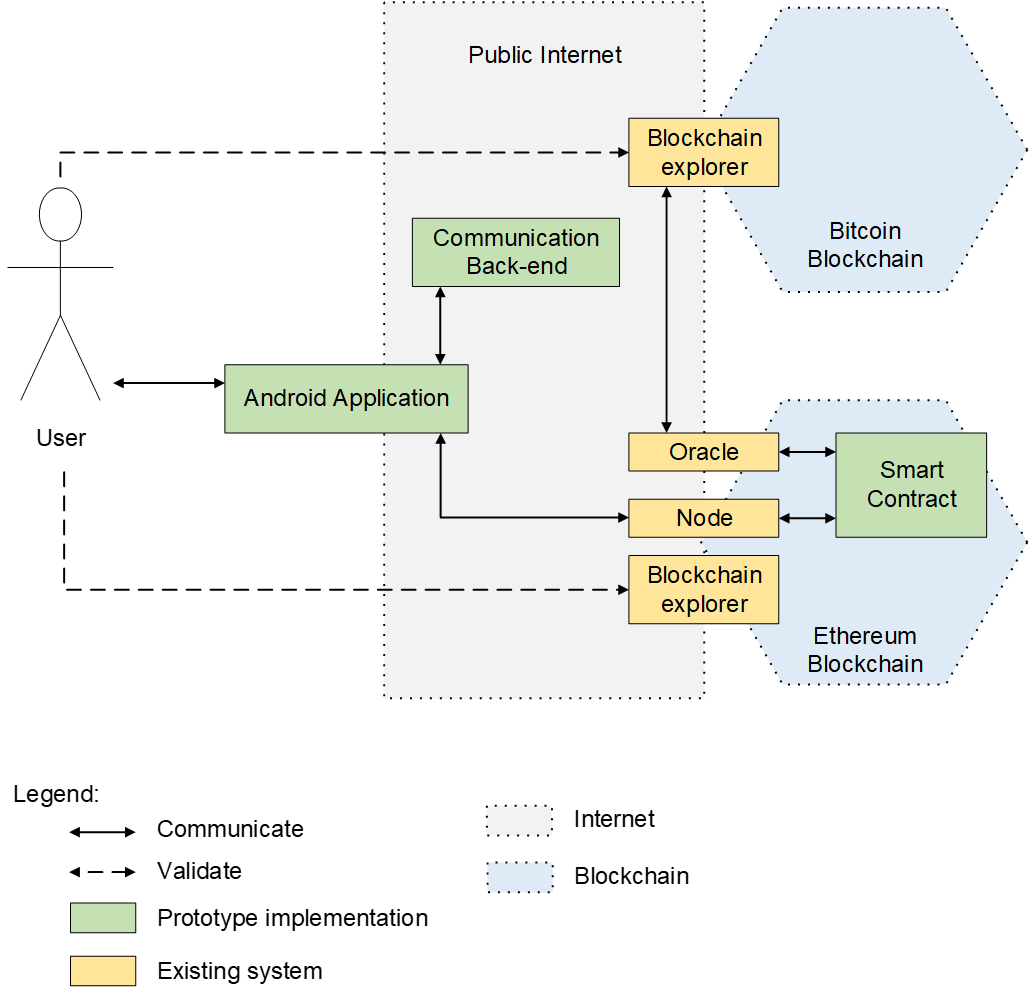
\includegraphics[width=\textwidth]{system-overview}
    \caption[itemize]{
    Overview of the system parts:
    \begin{enumerate*}[label=(\roman*)]
        \item \textit{User} communicates directly with the Android application and verifies data on the blockchain.
        \item \textit{Android application} fetches data about existing offers from the communication back-end and sends new smart contracts to the Ethereum node.
        \item \textit{Node} communicates with other nodes in the Ethereum network, maintains the status of the blockchain and deploys new smart contracts to the network.
        \item \textit{Smart contract} contacts oracle after deployment and holds the funds until the oracle has cleared the transaction as approved.
        \item The \textit{oracle} queries the Bitcoin block explorer to learn about the status of the transaction and communicates the result back to the smart contract.
    \end{enumerate*}
    }
    \label{fig:system-overview}
\end{figure}

\subsection{Requirements of system components}

//INTRO?

\subsubsection{Application front end}
The front end part of the proposed system has the task of receiving user's input and presenting the progress of a deployed transaction. It communicates directly with the node in order to deploy smart contracts and receive account balance and transaction hashes. Application receives data from the user (such as transaction value or destination address), verifies their validity and prepares the data in a format that can be consumed by the node. Front end also contacts the node and presents eventual replies to the user in an user-comprehensible format. If a reply is not received, the application needs to notify the user too.

\begin{figure}[ht]
    \begin{framed}
    \begin{tabular}{l l}
        \multicolumn{2}{c}{\textbf{Functional requirements}}\\
        \textbf{Requirement AF-1}&Verify user input.\\
        \textbf{Requirement AF-2}&Convert user input into node-compatible format.\\
        \textbf{Requirement AF-3a}&Deploy contract to the node.\\
        \textbf{Requirement AF-3b}&Query node for address balance.\\
        \textbf{Requirement AF-3c}&Query node for address nonce.\\
        \textbf{Requirement AF-4}&Display response from the node.\\
        
        \multicolumn{2}{c}{\textbf{Non-functional requirements}}
    \end{tabular}
    \end{framed}
   
    \caption{Caption}
    \label{fig:my_label}
\end{figure}

\subsubsection{Ethereum Node}
Ethereum node plays vital role in the application, as it deploys smart contracts, created by the user to the Ethereum network. If a node fails to do that, users cannot use the application for its purpose. We can say that the role of the node is \textit{business critical}.

The node needs to send transactions to the Ethereum network reliably and without delay. When queried, it must provide accurate and most up-to-date response. We can refer to these goals as trustworthiness and reliability. Since it is impossible to guarantee trustworthiness and reliability of any single node controlled by a third party, it would be in user’s best interest to operate their own node. However, operating a full node requires resources which may not be available on a mobile device.

If conditions do not allow for operation of a full node, second best alternative would be to query multiple nodes with the same request and accept the most common answer as the correct one. Since it is safe to suppose that majority of the nodes in the network are honest nodes, this would prevent single malicious node from affecting or halting the transaction process and would also resolve problems caused by downtime of any particular node. While this architecture certainly can be achieved, it is complex to fully implement such a scheme. The requirements 

\begin{figure}[ht]
    \begin{framed}
    \begin{tabular}{l l}
        \textbf{Requirement EN-1}&Send transactions to the network.\\
        
    \end{tabular}
    \end{framed}
   
    \caption{Caption}
    \label{fig:my_label}
\end{figure}

The consequences of nodes not fulfilling these requirements could be the impossibility to retrieve wallet balance and the impossibility to deploy contracts to the network, which would result in users not being able to use the application. Since the transaction for contract deployment is singed on user’s device, the node cannot alter transactions it receives. If user deployed a contract, but the node refused to provide transaction hash of this transaction, user’s trading partner would never transfer the second currency. The user would therefore waste funds on paying for the gas for the contract deployment, but would not lose funds as these would be transferred back after the contract timeout period has elapsed. //EXPLAIN ABOUT THIS/REFER TO EXPLANATION

\subsubsection{Smart contract}
The smart contract should implement the logic described in //DESCRIBED WHERE. It also must emit an event after construction as it is necessary for the user’s trading partner to verify that the contract was deployed as agreed. For its correct execution, it must also cater for any costs required to cover the services of an oracle. Application should reflect such costs in user interface, if this is the case.

Optionally, the contract can also emit an event when it receives a response from the oracle. If a transaction was not completed, such event could help users understand the reason.

Contracts should also be as short as possible to keep the costs of deployment and operation of the contract to minimum, as the user needs to pay for gas for every bytecode instruction. High prices of operating a contract could deter users from using the application.


\subsection{Implementation of system components}

//DUNNO? Section intro I suppose

\subsubsection{Application front end} 

To implement this functionality //functionality mentioned in XXX, the Android platform was chosen. Currently, it is the most used operating system in the world\footnotemark which ensures compatibility with significant number of devices. It is capable of carrying out the tasks outlined above and it does not require a centralised server to operate (as opposed to a website/web application). Development tools and documentation available free of charge and author's previous knowledge of Android programming were the further supporting arguments for Android. Android \acrshort{api} version 26 (Android Oreo) was chosen, as it is the newest supported version at the time of writing, although this has little practical implications. The prototype uses some user-interface features that were first introduced in \acrshort{api} version 22, so the minimal required Android version could be rolled back to this version without any changes.
% 
\footnotetext{\url{http://gs.statcounter.com/os-market-share}, as of 06-05-2018. See //REFERENCE TO APPENDIX for details}

In conjunction with Android, standard Java programming language was used. This is as opposed to Kotlin, a statically typed programming language, which was developed by JetBrains\footnotemark and pronounced the official Android programming language by Google on 17th May 2017 \cite{Vasic2017MasteringKotlin}. 
% 
\footnotetext{JetBrains is a company that created IntelliJ and other popular \acrshort{ide}s. \url{https://www.jetbrains.com/}}
% 
Many industry professionals suggest migrating to Kotlin as it offers several advantages \cite{Vasic2017MasteringKotlin} \footnotemark, but it has no direct implication on the prototype, as it compiles to the same byte-code as Java.
% 
\footnotetext{\url{https://medium.com/@magnus.chatt/why-you-should-totally-switch-to-kotlin-c7bbde9e10d5}, accessed 06-05-2018}

We will describe the structure of the prototype using the terminology of the \acrfull{modelvp} architecture pattern, which describe the architecture of an application in three layers or interfaces:
\begin{enumerate*}[label=(\roman*)]
    \item \textit{Model}
    \item \textit{View} and
    \item \textit{Presenter}
\end{enumerate*}.
The prototype does not fully succeed in following this patter, but it does share the major features with it. In the prototype, the split between model and presenter is not ideal and these two layers partially overlap. The approximation is as follows:
\begin{itemize}[noitemsep]
    \item Fragments have the role of the \textit{view} part
    \item \texttt{MainActivity} and wrapper classes have the role of the \textit{presenter} part
    \item \texttt{TradeDeal} and \texttt{BtcOffer} have the role of the \textit{model}.
\end{itemize}

\paragraph{View} The view part of the \acrshort{modelvp} is represented by eight fragment classes. Each fragment represents one screen of the application. XML files are used to describe the user interface elements of each fragment. Fragments read user inputs from these elements and update them accordingly with information recieved from \textit{presenter} interface. Example of such fragment is \texttt{DeployContractFragment}, which displays wallet balance in one \texttt{TextView} and reads user's input from another.

\paragraph{Presenter} 
\begin{sloppypar}
To navigate between fragments and update the view with new data, \texttt{MainActivity} is used. It implements interface \texttt{OnFragmentInteractionListener} that listens for user interaction in the fragments and responds accordingly. For example if the user selects to create a new offer by clicking on appropriate button, fragment calls the \texttt{onFragmentInteraction} method of \texttt{OnFragmentInteractionListener}, which is implemented in the activity class. \texttt{MainActivity} then initiates fragment transaction and replaces the old fragment with \texttt{CreateOfferFragment}.

The \textit{presenter} part of \acrshort{modelvp} is further complemented by three wrapper classes (\texttt{EthereumWrapper}, \texttt{BitcoinWrapper} and \texttt{FirebaseWrapper}). These classes contain methods to convert data to and from user-comprehensible format (e.g. method \texttt{satoshiToBtcString} from \texttt{BitcoinWrapper} class that converts the amount in satoshi to more user-friendly format -- decimal Bitcoins) and to communicate with the network (e.g. method \texttt{fetchExistingOffers} in \texttt{FirebaseWrapper} to get data from the database or method \texttt{sendContract} in \texttt{EthereumWrapper} to deploy contract to the network).
\end{sloppypar}

\paragraph{Model}
The \textit{model} interface in the prototype is represented by classes \texttt{BtcOffer} and \texttt{TradaDeal}. The first is used to contain all details of an offer to sell Bitcoins, both when a new offer is created and when existing offers are loaded from the database. When a user decides to proceed with an offer, \texttt{BtcOffer} is transformed into a \texttt{TradeDeal}. Trade deal holds further details of the offer, such as the deploying address and is used during the transaction validation process and during contract deployment.

The Java representation of the smart contract, \texttt{SmartExchange2} is also part of the model. It does not operate any logic in the Android application, but it holds the binary representation of the compiled Solidity code. The methods of this Java representation would also be used to communicate with an already deployed smart contract, although this functionality is currently not implemented in the prototype as it is not needed. \texttt{SmartExchange2} also contains the constructor used to pass initial value to the contract upon deployment. It is important to note, that \texttt{SmartExchange2} is an auto-generated code by the Web3j library, which takes ABI and BIN files of a compiled contract as the input and returns a single Java class as the output.

\subsubsection{Node}
As mentioned in //REFERENCE TO SECTION OF SOTA, Etherumj could be used to connect to the Ethereum network. However, running a full node on the Android platform may not be a viable solution, due to limitations of mobile devices. These limitations include storage, network bandwidth and power consumption. Fully connected node maintains a local copy of the blockchain (storage) and regularly communicates with the network peers to get the most recent block (network and battery consumption). Alternative solution to lower the load on the mobile device would be to run a light client (//GITHUB REFERENCE), which is targeted specifically for mobile devices and that does not maintain a local copy of the whole blockchain.

To speed up the development, we decided to use a remotely hosted node for this prototype. Instead of deploying own remote Ethereum node, a node-hosting service Infura was chosen. Upon creating an account on Infura’s website, developer is presented with a series of API endpoints – one endpoint for all major Ethereum networks (Mainnet, Kovan, Rynkeby…). Endpoints accept connections from any client and no authentication is needed. This is not an issue, since by design, the prototype signs the transaction on device, before it is deployed to the network, so the node does not have access to any sensitive data.

While running a single node is sufficient to demonstrate the idea of the prototype, more work should be put into implementing the solution with multiple nodes. In a market-ready version of the application, the centralisation implied by using a single node would pose as a major, business critical drawback. This should be one of the first issues to address in any further development of the application.
% 
\subsubsection{Smart Contract}
The contract was written in the Solidity language, as it is currently the recommended (//?) language for smart contracts. The latest available version //SOLIDITY VERSION (probably newest) was used. The smart contract was written using Remix, an in-browser IDE, recommended for use with Solidity, which enables sandbox contract testing. Oraclize (//EXPLAIN WTH IS ORACLIZE) version of Remix was also used to test the functionality of an oracle.

Smart contract in Solidty was then compiled into binary and ABI (//EXPLAIN WHHAT THIS) files, using the solc compiler. The BIN and ABI files where then used by Web3j command line tools to generate Java representation of the Smart contract (//LINK TO FILE IN ATTACHMENT/APPENDIX). On top of the compiled smart contract in binary form, this Java file also includes wrapper methods to invoke the custom constructor and the methods of the contract.

% 
\subsubsection{Oracle}

Using Oraclize for this service... why? Why not?
% 
\subsubsection{Blockchain explorer}
Using blockchain.info... why? Why not?

\subsubsection{Database //Firebase}
The back end for user communication is mostly included in the prototype to demonstrate the flow of the transaction. While in the prototype implementation, the communication back-end is necessary to coordinate actions of primary and secondary user, in a market-ready product it should only play supportive role -- so that even when the back-end is not operational, the application still can be used.


\paragraph{Drawbacks}
Using 1 node in the prototype

Using oraclize in the prototype

Using blockchain.info in the prortytype

Using unsecured database in the prototype.

\subsection{Evaluation}\label{sec:evaluation}

In the following sections, we evaluate the implemented system. We compare our implementation of the system against the system requirements established in Section~\ref{sec:system-reqs} (p. \pageref{sec:system-reqs}) and then compare individual system components against their respective requirements (Section~\ref{sec:component-reqs}, p. \pageref{sec:component-reqs}). For every requirement we review, whether it was implemented fully, partially or not at all and asses, what implications does not implementing this requirement have on the overall system. Afterwards, a model transaction will be performed on test networks, using two Android devices.

\subsubsection{Requirement implementation evaluation}

We were able to implement all of the functional and two non-functional system requirements. We did not succeed in fully implementing one non-functional requirement -- PT-NFR-2 in particular. This requirement specifies that there should not be a single point of failure in the system. There are several places in the system, where this requirement is not adhered to. The prototype application only communicates with one single Ethereum node (single Infura instance), the deployed smart contract only contacts one oracle (Oraclize) and the oracle only contacts one blockchain explorer service (Blockchain.info). If any of these providers went offline, the system could not make transactions. Table~\ref{tab:system-reqs-eval} provides an overview over system requirements. Similar table elaborating on requirements of individual system components can be found in Appendix~\ref{sec:appendix-table} (p. \pageref{sec:appendix-table}).

\begin{table}[ht]
    \centering
    \begin{tabularx}{\textwidth}{|l X c|}
    \hline
    \textbf{ID}&\textbf{Description}&\textbf{Implemented}\\
    \multicolumn{3}{|l|}{\textbf{Functional requirements}}\\
    PT-FR-1 & The primary user and the secondary user should be able to agree on the terms of the transaction.&Yes\\
    PT-FR-2 & The primary user must be able to deploy a smart contract to the Ethereum network.&Yes\\
    PT-FR-3 & The secondary user should be able to verify contract deployment.&Yes\\
    PT-FR-4 & The secondary user should be able to transfer Bitcoin.&Yes\\
    PT-FR-5 & If the secondary user does not transfer Bitcoin, the primary user must receive their Ether back.&Yes\\
    PT-FR-6 & Primary user and secondary user must be ably to verify the status of their transaction.&Yes\\
    \multicolumn{3}{|l|}{\textbf{Non-functional requirements}}\\
    PT-NFR-1&The system must implement architecture proposed in Figure~\ref{fig:arch-ver2-tech}.&Yes\\
    PT-NFR-2&There should not be single point of failure in the system.&\textbf{No}\\
    PT-NFR-3&No other party should have control over the funds of primary user and secondary user.&Yes\\
    \hline
    \end{tabularx}
    \caption{Overview over system requirements. One requirement was not successfully implemented.}
    \label{tab:system-reqs-eval}
\end{table}

Ideally, the application would have a list of back-up nodes which it can contact in case that the primary node is unresponsive. Furthermore, the application should consult these back-up nodes to verify, that the primary node deployed the transaction to the network. The back-up nodes should be from different providers and preferably hosted at different locations. Only this way, the users can be certain that there is no single party having influence over these nodes. This requirement was not implemented in the first version of the system due to technical challenges and costs associated with deploying and/or connecting to a series of Ethereum nodes and due to the fact, that the idea initial can be successfully demonstrated with single Ethereum node. Non-functional requirements EN-NFR-1, EN-NFR-2 and EN-NFR-3, which specify the performance of the Ethereum node in terms of honesty and trustworthiness are not marked as \textit{Fulfilled}, since it is not possible to enforce these qualities in a single node. If a solution with back-up nodes was implemented, these requirements would not be relevant anymore.

Similarly, the smart contract only queries one oracle (Oraclize) and this oracle queries one blockchain explorer (Blockchain.info). If either the oracle or the blockchain explorer goes offline or deliberately provides incorrect responses, the transaction would not execute correctly. Neither the oracle nor the blockchain explorer do not directly control user's funds, but if they deliberately provided a false answer to the smart contract (e.g stating that the balance on the queried address is higher than it actually is), the transaction would not execute correctly. In the given example, the secondary user would receive Ether from the smart contract, even though they did not uphold their part of the agreement and did not transfer the Bitcoins. Ideally, to remove dependency on a single provider, the smart contract should query several independent oracles, with a different blockchain explorer as the target in every query. In case different responses are received, smart contract would need to decide which response to pick as the correct one (probably the most common one). If this was the case, requirements OR-NFR-1, OR-NFR-2, BE-NFR-1 and BE-NFR-2 would lose their relevance.

The prototype version of the system does not implement this, as currently there are not enough providers offering services of an oracle, that could be used. Some competitors of Oraclize either went out of business (case of Tinypay.co\footnote{\url{https://medium.com/@mustwin/building-an-oracle-for-an-ethereum-contract-6096d3e39551}, accessed 19-05-2018}) or do not offer the desired functionality -- contacting a web API (case of RealityCheck\footnote{\url{https://github.com/realitykeys/realitycheck}, accessed 19-05-2018}). We did not attempt to deploy our own oracle, as this is not the scope of this project.

Another requirement which was not fully implemented is the requirement SC-NFR-2, which states that smart contract must cover the costs for the services of the oracle. This requirement is not relevant in current implementation, as Oraclize does not charge any fees for the first query made from a smart contract. Since a new smart contract is deployed with every transaction and with current system there is only one query made right after the contract was created, no fees for the oracle are needed. However, if Oraclize changed their fees or if another provider was used, smart contract would need to be adapted for this.

Last requirement which was not implemented is the requirement CB-NFR-1. This is marked as \textit{Not implemented}, because in the prototype, users are not able to proceed with the transaction, unless the transaction status code has been update in the database. The current prototype does not accommodate users that agree on the terms of the transaction via another channel than the application itself. This behaviour could be easily changed by adapting the user interface of the application and allowing user to proceed with the transaction without consulting the transaction progress with the database.
%
%
%
%
%
%%%%%%%%%%%%%%%%%%%%%%%%%%%%%%%%%%%%%%%%%%%%%%%%%%%%%%%%%%%%%%%%%%%%%%%%%%
\subsubsection{Example of a transaction scenario}
In this experiment we demonstrate a transaction between two fictitious people -- a primary user Eve, who wants to sell Ether and buy Bitcoin, and secondary user Mike, who wants to buy Ether and sell Bitcoin. Both users are running the application on their phones. Eve has her own Ethereum wallet with some Ether she wishes to sell. Mike has his own Bitcoin wallet he will use to make the transaction. Eve's and Mike's wallets are standalone systems, independent from our system. The scenario of the transaction is outlined in Figure~\ref{fig:transaction-scenario}. 

\begin{figure}[ht]
    \centering
    \begin{framed}
    \begin{enumerate}[noitemsep]
        \item Mike creates a Bitcoin offer in the application by inputting:
            \begin{itemize}[nolistsep,noitemsep]
                \item Amount in Bitcoin he wishes to sell.
                \item Amount in Ether he wishes to receive.
                \item Ethereum address, where he wishes to receive the Ether.
            \end{itemize}
            Mike then and publishes this offer in the database.
        \item Eve selects this offer and transfers Ether to a temporary Ethereum address.
        \item Eve then creates an empty Bitcoin address and inputs this address into the application.
        \item A smart contract is deployed from the temporary address with following properties:
            \begin{itemize}[nolistsep,noitemsep]
                \item Mike's Ethereum address.
                \item Eve's Bitcoin address.
                \item Amount of Bitcoin, Eve and Mike are trading.
            \end{itemize}
            Besides these properties, which are specified in the smart contract constructor as data fields, the creation of a contract also carries two other significant information:
            \begin{itemize}[nolistsep,noitemsep]
                \item Sender's Ethereum address -- this is used to return the funds in case of unsuccessful transaction.
                \item Value, associated with the transaction -- this is the amount of Ether that Eve and Mike are trading.
            \end{itemize}
        \item After the smart contract has been deployed, Mike verifies correctness of the information in it. If all information are correct, Mike transfers Bitcoin to Eve.
        \item The oracle responds to a query sent by smart contract. Based on this response, smart contract sends its Ether balance either to Mike (in case of successful transaction) or to Eve (in case of unsuccessful transaction).
    \end{enumerate}
    \end{framed}
    \caption{Scenario of a transaction between Eve and Mike.}
    \label{fig:transaction-scenario}
\end{figure}

We successfully executed this scenario using two Android devices, a Parity Ethereum wallet and a GreenAddress Bitcoin wallet. The transactions were made on Ethereum \textit{Kovan} test network and Bitcoin \textit{testnet3} test networks. Eve's device was a OnePlus A5000 running Android 8.1.0 Oreo. Mike's device was a Samsung AM-A510F, running Android 7.0.0 Nougat. Both devices were connected to a mobile network and were sharing their screens with a computer via \acrshort{adb}. The whole process took approximately 20 minutes, out of which 10 minutes is the oracle response delay. The cost of the smart contract deployment was approximately 0.05 kETH\footnote{\textit{kETH} is used to indicate Kovan Ether.} and was paid by Eve\footnotemark. Table~\ref{tab:trade-story} describes the experiment progress step-by-step. Figure~\ref{fig:screenshot-contract} (p. \pageref{fig:screenshot-contract}) shows the application screen after the smart contract has been sent to the network. In Appendix~\ref{sec:appendix-screenshots} (p. \pageref{sec:appendix-screenshots}) we include complete list of screenshots taken during the experiment and their description. We can conclude, that successful execution of this scenario proves, that the proposed system is operational and can be used for~its~purpose.
% 
\footnotetext{We elaborate further on the cost of the transaction in the Discussion chapter (p. \pageref{sec:discussion}.)}

\newgeometry{left=0.5cm,right=.5cm,top=.5cm,bottom=1cm,footskip=.4cm}
\begin{table}[ht]
    \centering
    \begin{tabularx}{\textwidth}{|c|X|X|}
        \hline
        \textbf{Step}&\textbf{Eve}&\textbf{Mike}\\
        \hline
        1&Opens the application.&Opens the application.\\
        \hline
        2&Sees, that there are currently no available offers.&Clicks on \textit{Create new offer}.\\
        \hline
        3&&Fills in the amount of Bitcoin he wishes sell and amount of Ether he wishes to buy.\\
        \hline
        4&&Uses QR code scanner to input the address of his Ethereum wallet.\\
        \hline
        5&&Clicks on \textit{Create new offer}. This sends the offer to the database.\\
        \hline
        6&A new offer is added to the list. Eve selects this offer and clicks \textit{Confirm}.&Is presented with a screen showing the status of his offer.\\
        \hline
        7&A temporary address, from which the contract will be deployed, is presented to Eve. She has a choice to use this temporary address or import her own. She decides to use the temporary address.&\\
        \hline
        8&She transfers the amount of Ether to sell to the temporary address.&\\
        \hline
        9&A screen with further details is presented to Eve. Mike's Ethereum address and amount of Bitcoins are pre-filled. She creates a new empty Bitcoin wallet and enters its public address to the application. This is where Mike will send his Bitcoins.&\\
        \hline
        10&Eve uses the QR scanner to fill in her Bitcoin address and then clicks on \textit{Validate}.&\\
        \hline
        11&Validation screen is presented to Eve. The \textit{Yes} button is greyed out and she cannot click it yet.&Confirmation screen is presented to Mike informing him, that someone is interested in his offer. Mike presses \textit{Yes}.\\
        \hline
        12&The \textit{Yes} button on the confirmation screen now turns blue. Eve clicks it.&Message on Mike's screen informs him, that he confirmed the offer and is waiting until the other party responds.\\
        \hline
        13&\multicolumn{2}{|>{\hsize=2\hsize}X|}{\centering The smart contract is now deployed to the network. As a confirmation, a link to a Blockchain explorer is presented to both users. The smart contract contacts an oracle with a query carrying Eve's Bitcoin address.}\\
        \hline
        14&&Mike verifies the contract using a blockchain explorer and then clicks \textit{Continue}\\
        \hline
        15&&A new screen informs him, where he needs to send the Bitcoin.\\
        \hline
        16&&Mike transfers Bitcoin to specified address, using a Bitcoin wallet, which is not part of the system.\\
        \hline
        17&Eve receives the Bitcoin.&After 10 minutes, the oracle responds to the query of the smart contract. Smart contract compares the balance on the monitored address with the balance in its memory. Since they match (Mike transferred the right amount of Bitcoin), it sends its Ether balance to Mike's Ethereum address.\\
        \hline
        18&Eve has received Bitcoin.&Mike has received Ether.\\
        \hline
        \multicolumn{3}{|>{\hsize=2\hsize}c|}{The transaction is completed.}\\
        \hline
    \end{tabularx}
    \caption{Execution of the trading scenario with two fictitious users.}
    \label{tab:trade-story}
\end{table}
\restoregeometry

\begin{figure}[ht]
    \centering
    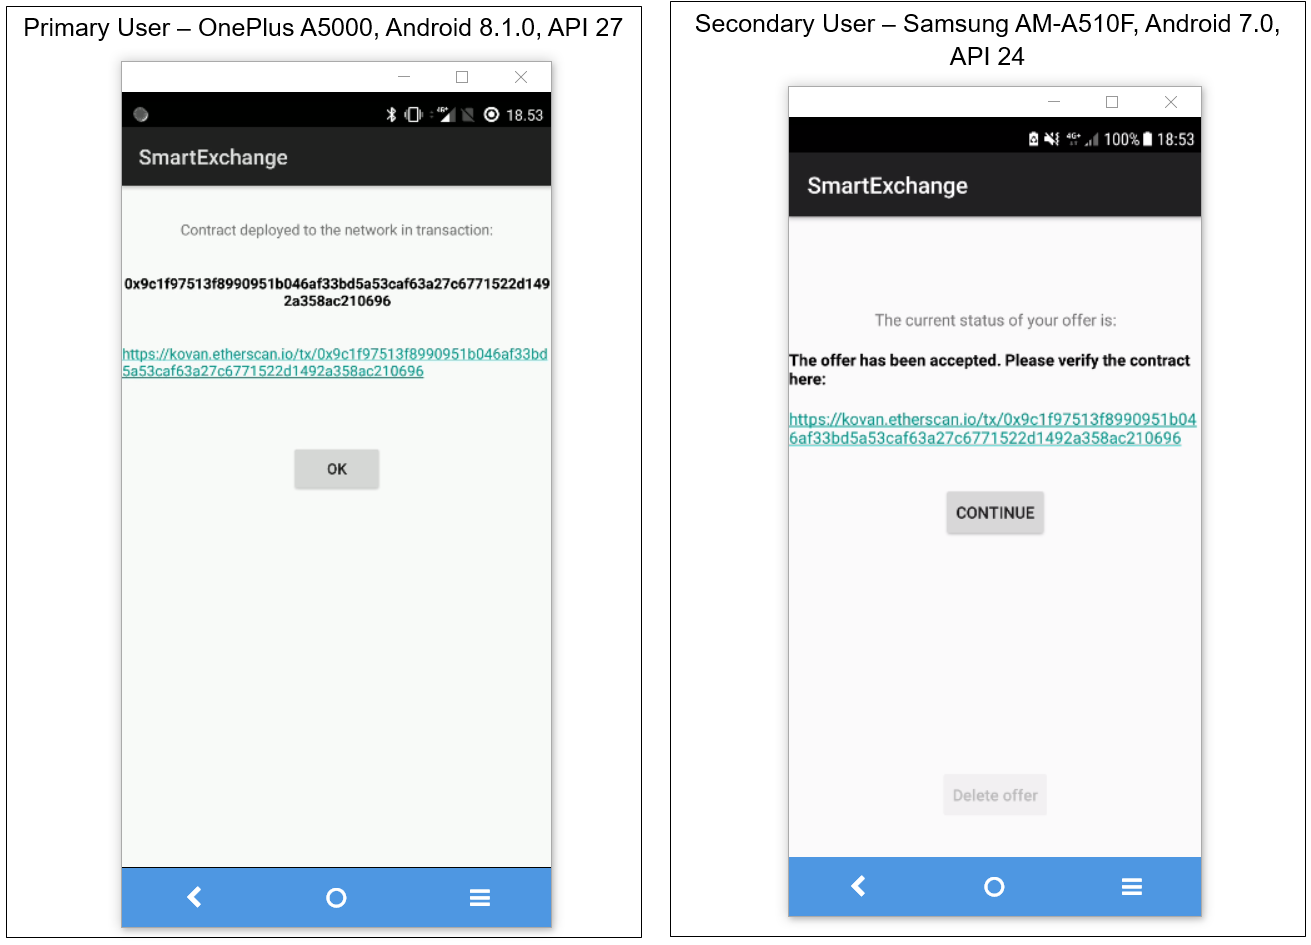
\includegraphics[width=\textwidth]{screenshots/screen091}
    \caption{Screen of both instances of the application, after the smart contract has been deployed to the network. Eve is on the left.}
    \label{fig:screenshot-contract}
\end{figure}
%
%
%
%
%
%%%%%%%%%%%%%%%%%%%%%%%%%%%%%%%%%%%%%%%%%%%%%%%%%%%%%%%%%%%%%%%%%%%%%%%%%%
\subsubsection{Known weaknesses}
The sample scenario demonstrated, that the system enables two users to trade Ether and Bitcoin with the use of a smart contract. However, we must note that this scenario was carried out under ``sunny day conditions''. There was no risk of losing any real currency, since the experiment was carried out on a test network. There was no attacker, attempting to disrupt the transaction process and the external services used (Infura, Oraclize, Blockchain.info and Etherscan) were all operational and honest. The two fictitious users were controlled by the developers, thus they had absolute knowledge about the system and were certain about the various features of the application and about the user interface components. Most of these issues were not addressed due to the time constrains, even though some could be solved easily.

We do realise, that this is not always the case and any of these conditions can be violated during regular use. In following paragraphs we describe some of the most severe issues of the system. While the system can still be used, as demonstrated above, if exploited, these issues could lead to the system being unusable or funds being lost in the worst case. These issues should be addressed in further development.

\paragraph{Use of only one node}
The system at its current state only uses a single Infura node. The node does not have control over users funds, since the transactions are signed offline (in the Android application). However, the node could still refuse to send a transaction to a network and this way influence the transaction process. Similar issue persists, if the provider goes offline -- no users would be able to make transactions,

While running a single node is sufficient to demonstrate the idea of the prototype, more work should be put into implementing the solution with multiple nodes. In a market-ready version of the application, the centralisation implied by using a single node would pose as a major, business critical drawback.
% 
\paragraph{Use of only one oracle and blockchain explorer}
As noted previously, the system only uses one oracle and one blockchain explorer provider. Similarly as the Infura node, they could prevent transactions from happening, if either of the two goes offline. Additionally, the blockchain explorer and the oracle can also provide counterfeit data to the smart contract. Either of the two could alter the response to the smart contract, altering the balance on the queried account and therefore influence the behaviour of the smart contract. Using the model scenario as an example, if Mike had not transferred the Bitcoin, but instead manipulated the Blockchain.info, that the queried account does have the balance he was supposed to send, then the smart contract would release the funds to him. In similar fashion he could hypothetically manipulate the oracle, yielding the same result.

A solution, where multiple oracles are queried with different blockchain explorers could make it more difficult to execute the above attack.
% 
\paragraph{Unsecured access to the database}
Firebase allows several options how to restrict the read and write access to the database. With the current setup however, anyone who has the database reference string (database URL) can read and write all data in the database. This is obviously not secure, since anyone could retrieve the string from the application source code and flood the database with bogus offers or delete all existing real offers. The access to the database should be limited, so that this malicious activity is prevented. This could be done by only allowing users to change offers they created and only allowing them to create a limited number of offers per hour. This issue needs to be addressed in the further releases of the application.

\paragraph{Database controls the transaction flow}
The current process of making a transaction is tied to the \texttt{offerStatus} codes received from the database. If users do not wish to interact through the database and decide to use another communication channel outside our system, the application should be able to handle this. Currently, however it does not allow to deploy a contract directly and all the transactions need to be created in the database, before they are picked up by the application.

This functionality should be fixed in the application, where users should be able to deploy a smart contract manually (i.e. where the user selling Ether manually enters all the required data).
% 
\paragraph{User interface flaws}
There were no requirements established for the user interface, nor did the user interface undergo any user testing. There are some flaws in the user interface that make the application confusing to use. This was not addressed in this project as it is out of scope, but should be revisited in further development.

Moreover, due to rather complicated transaction process (Figure \ref{fig:arch-ver2-tech}, p. \pageref{fig:arch-ver2-tech}) and importance of carrying out the steps in the correct order to maintain the desired level of security, the user should be presented with a guide upon the first application launch, which would describe the steps and guide the user through the process of making a transaction.

\paragraph{Ether return policy}
In the prototype, user needs to use the temporary address, generate by the application, as the \textit{Import wallet} function has not been implemented. In case the secondary user does not transfer Bitcoin as agreed, the Ether funds would be returned to this temporary address. The application currently does not display private key of this temporary address, therefore the user is not able to access the returned funds. It is possible to use these funds to make another transaction, but the temporary address is lost when the user closes the application. This is an application flaw and should be fix be redesigning the user interface.

\subsection{Conclusion}

In this chapter we have identified the necessary components to support our desired transaction process, specified in the \textit{System Design} chapter. We specified functional and non-functional requirements for the system as a whole and for the individual components. We presented the final version of the architecture that we later implemented. We described implementation of all the parts and how they interact together.

In the \textit{Evaluation} section we have verified that the implemented system fulfils the requirement outlined earlier. We than proceeded to test the operation of the system in the model scenario. We can conclude that the implemented prototype is capable of carrying out the desired transaction, which was demonstrated in the scenario. At the end of this chapter we listed some known issues that would need to be addressed in the further development of the system. In the following chapter \textit{Discussion}, we debate the outcomes of the project.